
\subsection{link-analysis}\label{sec:tuning:link}

Neither \textit{eswc2015movies} nor \textit{eswc2015music} was runnable with \textit{link-analysis} on the test setup so they are excluded from this discussion.

What follows is a description of the different optimization strategies evaluated:

\begin{description}
    \item[grid]
        Does a grid search over a subset of $\gamma$ and $\eta$, given a fixed step size. $-10 \leq \gamma \leq 10$ x $-10 \leq \eta \leq 10$ was examined with a step size of 1.
    %\item[rand]
        %Randomly samples over a subspace of $\gamma$ and $\eta$, given a fixed number of samples.
    \item[adapt-hill]
        A hill climbing algorithm over both $\gamma$ and $\eta$. It starts with a fixed step size and compares the neighbours. If a local optima is found, the step size is decreased. Continues until a specified function, eta or gamma tolerance has been reached. An initial step size of 1 is used and a $\eta$ tolerance of 1 and a $\gamma$ tolerance of 0.5 is used. The algorithm aborts whenever a function tolerance of $< 0.01$ is reached.
    \item[adapt-hill-gamma]
        Similar to \textbf{adapt-hill}, but instead of searching over $\eta$ it keeps $\eta = 1$ and optimizes over $\gamma$. When a local optima is found, $\eta = -1$ is tried.
    %\item[sim-ann]
        %Simulated annealing over $\gamma$. Try $\eta = 1$ and $\eta = -1$.
\end{description}


\begin{figure}[h!]
    \centering
    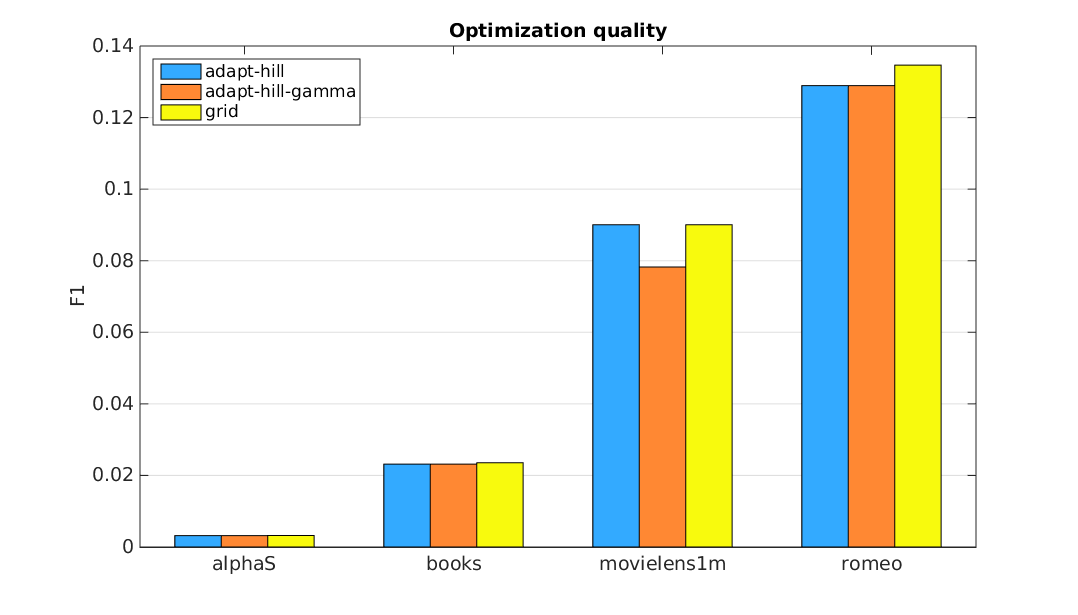
\includegraphics[width=0.9\textwidth]{fig/comp/comp_link_quality.png}
    \caption{Comparison of the recommendation quality given from the parameters found by thedifferent optimization strategies for \textit{link-analysis}.}
\end{figure}

The only difference between \textbf{adapt-hill} and \textbf{adapt-hill-gamma} can be seen with \textit{movielens1m}. Both display similar recommendation quality as the full grid search.

\begin{figure}[h!]
    \centering
    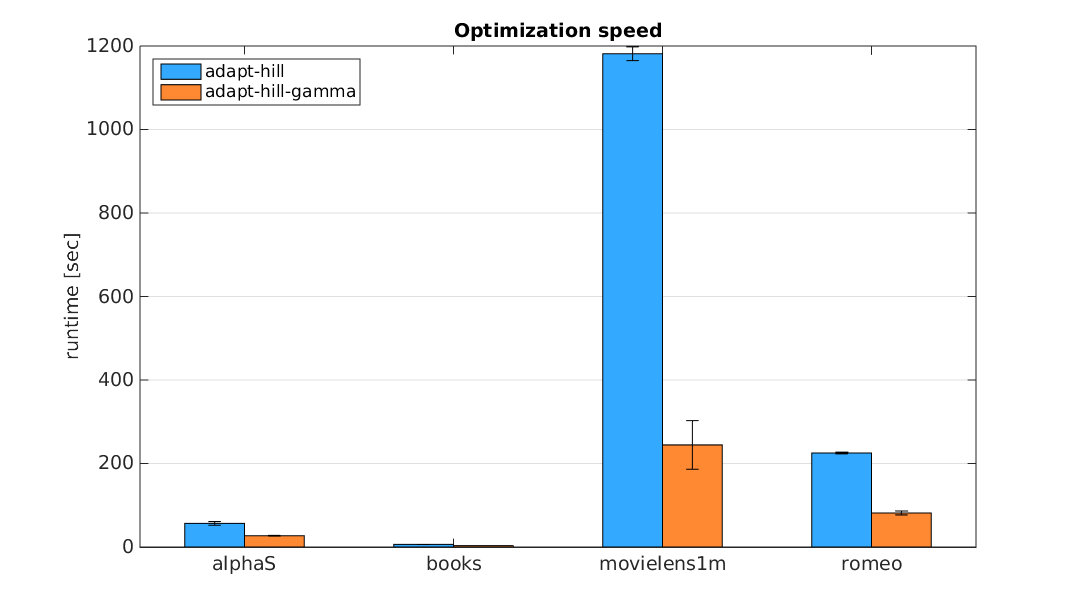
\includegraphics[width=0.9\textwidth]{fig/comp/comp_link_speed.png}
    \caption{Comparison of the runtime of the different optimization strategies for \textit{link-analysis}, given the optimized parameters specified in \appendixref{app:opt_params}.}
\end{figure}

\begin{figure}[h!]
    \centering
    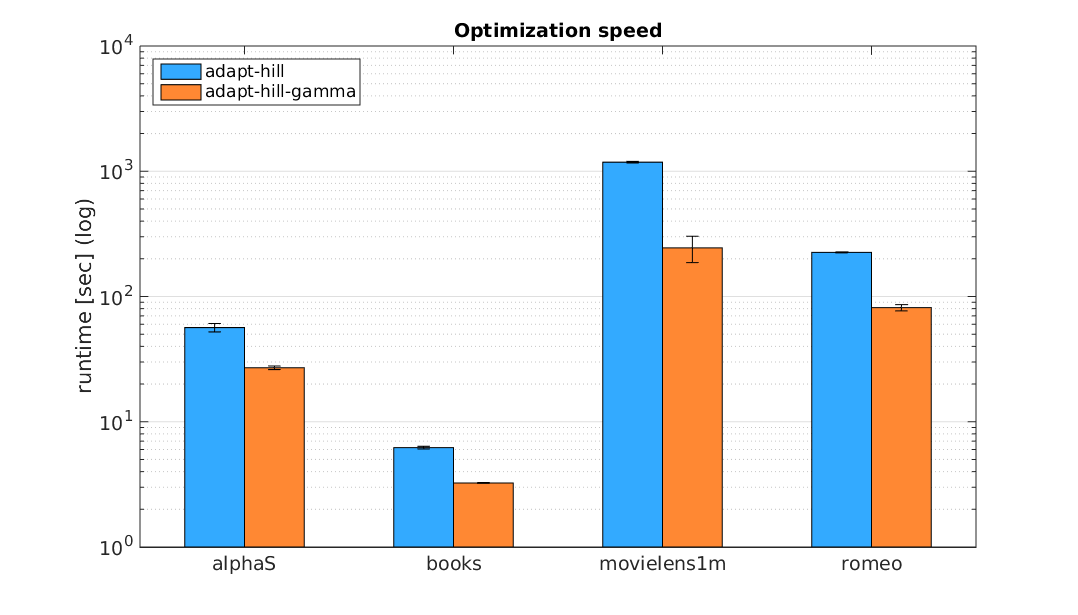
\includegraphics[width=0.9\textwidth]{fig/comp/comp_link_speed_log.png}
    \caption{Comparison of the runtime of the different optimization strategies for \textit{link-analysis}, given the optimized parameters specified in \appendixref{app:opt_params}. In a log scale.}
\end{figure}

\FloatBarrier

Grid search isn't shown in the runtime plots as it is too slow, for \textit{movielens1m} a runtime of approximately 6 hours is needed.  The runtime difference between optimizing over both $\gamma$ and $\eta$ compared to only optimizing over $\gamma$ is large while the difference in recommendation quality is negligible. This shows that purely optimizing over $\gamma$ using a hill climbing algorithm is better than the alternatives.

